\chapter{Abstraction turns problems and concepts into principles}
\label{chap:relationsandfunctions}


\begin{figure}[ht]
\centerline{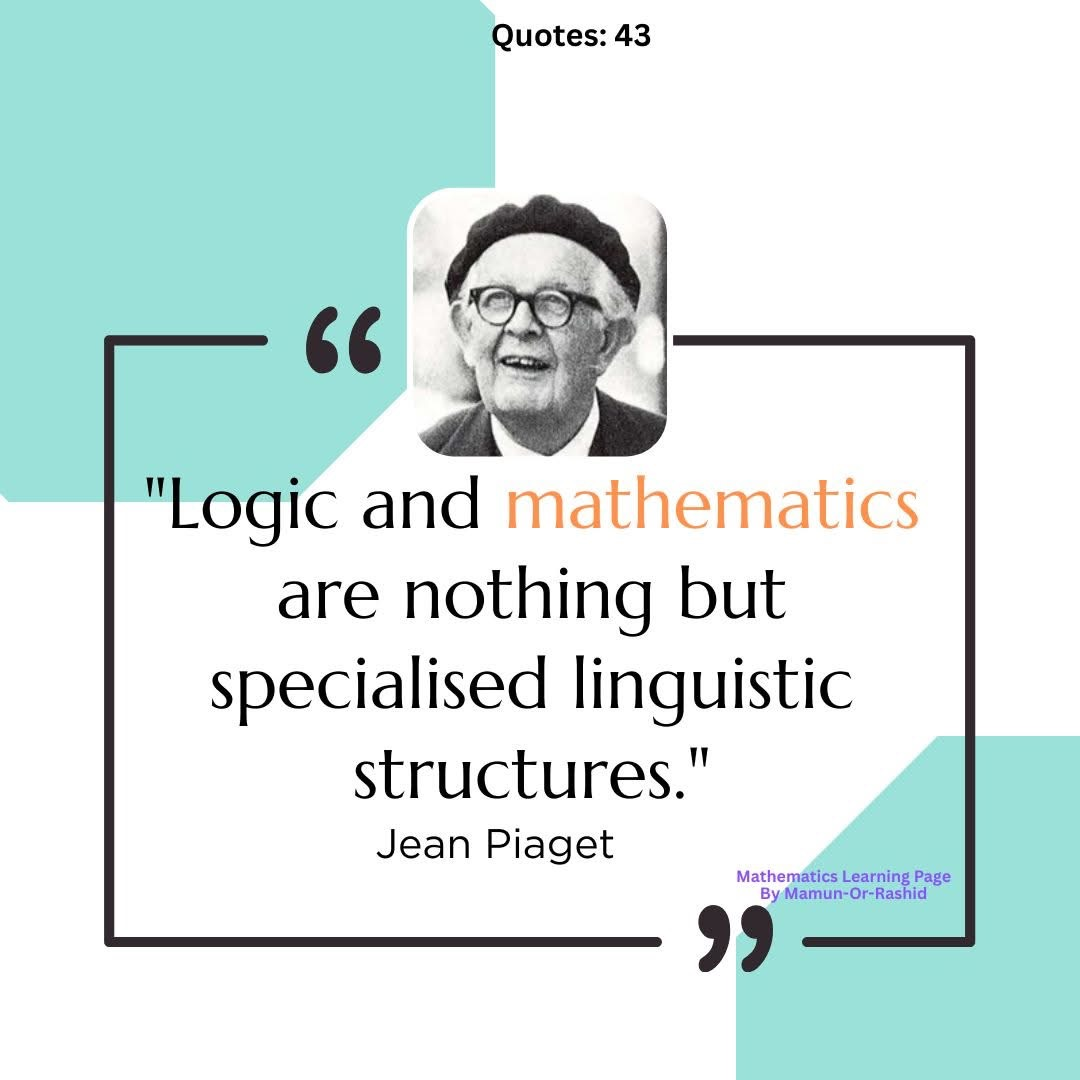
\includegraphics[width=2.0in]{images/piaget.jpg}}
\end{figure}

Modern mathematics and computer science are built upon a few simple but very powerful ideas. 
Among the most important are the notions of \emph{relations} and \emph{functions}, which 
allow us to describe how objects are connected or transformed. 
Counting, infinity, and the ways in which sets can be grouped into classes 
help us measure size, structure, and complexity. 
These ideas may look abstract at first, but they underlie the methods used 
in algorithms, data structures, and logical reasoning.

In computer science, functions capture the essence of computation: 
a program takes inputs and produces outputs, just as a function does. 
Understanding one-one and onto functions helps us reason about 
whether information is lost, preserved, or fully covered. 
Equivalence classes and partitions allow us to organise data into categories. 
Modular arithmetic, often called ``clock arithmetic,'' is fundamental 
in cryptography, error detection, and digital systems. 
Learning these concepts gives us a foundation to explore deeper 
mathematics and to apply it to practical computational problems.

\section{Relations}

The {\em Cartesian product} of two sets $A$ and $B$, denoted by
$A \times B$, is the set of all ordered pairs $(a,b)$ such that
$a \in A$ and $b \in B$. Thus,
\[
A \times B = \{(a,b) \mid (a \in A) \mbox{ and } (b \in B)\}
\]
$A^n$ is the set of all ordered $n$-tuples $(a_1,a_2,\ldots,a_n)$
such that $a_i \in A$ for all $i$. i.e.,
\[
A^n = \underbrace{A \times A \times \cdots \times A}_{n \mbox{ times}}
\]


A \emph{relation} tells us which elements of one set are connected to elements of another.

A {\em binary relation} $R$ from $A$ to $B$ is a subset of $A \times B$. It is
a characterisation of the intuitive notion that some of the elements of $A$ 
are related to some of the elements of $B$. 

If $A=\{1,2,3\}$ and $B=\{a,b,c\}$, then
$R=\{(1,a),(2,b),(3,a)\}$ is a relation from $A$ to $B$.
Familiar binary relations from
$\N$ to $\N$ are $=,\;\neq,\;<,\;\leq,\;>,\;\geq$. Thus the elements
of the set $\{(0,0),(0,1),(0,2),\ldots,(1,1),(1,2),\ldots\}$ are all members
of the relation $\leq$ which is a subset of $\N \times \N$.

\begin{figure}
\begin{center}
\begin{tikzpicture}[>=Stealth, node distance=10mm]
  % Left: relation that is not a function
  \node[draw, rounded corners, minimum width=3.2cm, minimum height=3.6cm,label=above:{\footnotesize Relation (not a function)}] (L) {};
  \node (A1) at ([xshift=-1.1cm,yshift=1.0cm]L.center) {$1$};
  \node (A2) at ([xshift=-1.1cm,yshift=0.0cm]L.center) {$2$};
  \node (A3) at ([xshift=-1.1cm,yshift=-1.0cm]L.center) {$3$};
  \node (B1) at ([xshift=1.1cm,yshift=1.0cm]L.center) {$a$};
  \node (B2) at ([xshift=1.1cm,yshift=0.0cm]L.center) {$b$};
  \node (B3) at ([xshift=1.1cm,yshift=-1.0cm]L.center) {$c$};
  \draw[->] (A1) -- (B1);
 % \draw[->] (A1) .. controls +(-0.2,-0.5) and +(0.2,0.5) .. (B2); % two outputs from 1
  \draw[->] (A1) -- (B2);
  \draw[->] (A2) -- (B3);

  % Right: valid function
  \node[draw, rounded corners, minimum width=3.2cm, minimum height=3.6cm, right=2.8cm of L,label=above:{\footnotesize Function}] (R) {};
  \node (C1) at ([xshift=-1.1cm,yshift=1.0cm]R.center) {$1$};
  \node (C2) at ([xshift=-1.1cm,yshift=0.0cm]R.center) {$2$};
  \node (C3) at ([xshift=-1.1cm,yshift=-1.0cm]R.center) {$3$};
  \node (D1) at ([xshift=1.1cm,yshift=1.0cm]R.center) {$a$};
  \node (D2) at ([xshift=1.1cm,yshift=0.0cm]R.center) {$b$};
  \node (D3) at ([xshift=1.1cm,yshift=-1.0cm]R.center) {$c$};
  \draw[->] (C1) -- (D1);
  \draw[->] (C2) -- (D2);
  \draw[->] (C3) -- (D2);
\end{tikzpicture}
\end{center}
\caption{Relation vs function: In a relation, an element in $A$ can be mapped to multiple elements in $B$, but not so in a function. In a function, all elements in $A$ must be covered, but not necessarily so in a relation. The set $B$ need not be fully covered in either. }
\label{fig:relationvsfunction}
\end{figure}

\section{Function}
A \emph{function} from $A$ to $B$ -- written as $f: A \to B$ -- is a special relation in which:
\begin{enumerate}
  \item every element of $A$ is related to some element of $B$, and
  \item no element of $A$ is related to more than one element of $B$.
\end{enumerate}
Equivalently, each input has \emph{exactly one} output. 

Some familiar examples of functions are 
\begin{enumerate}
\item   $+$ and $*$ (addition and multiplication) are functions of the type
        $f: \N \times \N \rightarrow \N$ 
\item   $-$ (subtraction) is a function of the type $f: \N \times \N \rightarrow
 \Z$.
\item   $div$ and $mod$ are functions of the type $f: \N \times \N \rightarrow \N$.
        If $a = q*b + r$ such that $0 \leq r < b$ and $a,b,q,r \in \N$ then
        the functions $div$ and $mod$ are defined as $div(a,b) = q$ and
        $mod(a,b) = r$. We will often write these binary functions as
        $a * b$, $a\; div \;b$, $a \; mod \; b$ etc.
\item   The binary relations $=,\;\neq,\;<,\;\leq,\;>,\;\geq$ are also functions of the type
        $f: \N \times \N \rightarrow \B$        where $\B = \{false,true\}$.
\item $f:\N\to\N,\ f(x)=x^2$.
\end{enumerate}


We write the definition of a function formally as follows.

A {\em function} from $A$ to $B$ is a binary relation $f$ from $A$ to $B$ such
that for {\em every} element $a \in A$ there is a {\em unique} element
$b \in B$ so the $(a,b) \in f$ (or $f(a) = b$)\footnote{This is sometimes written using mathematical notation as $\forall a \in A$, $\exists$ unique $b \in B$. $\forall$ is the usual symbol for {\em for all}, and $\exists$ is the usual symbol for {\em there exists}}. We will use the notation 
$f: A \rightarrow B$
to denote a function $f$ from $A$ to $B$. The set $A$ is called the 
{\em domain} of the function $f$ and the set $B$ is called the {\em co-domain}
of the function $f$. The {\em range} of a function $f: A \rightarrow B$ is the
set $\{b \in B \mid \mbox{for some $a \in A$, $f(a) = b$}\}$ denoting the subset of elements in $B$ that are actually covered by $f$. 


\subsection{One-One (injective), Onto (surjective), and bijective Functions}
When we study functions, it is often not enough to know that “every input has exactly one output.”
We also want to understand how well the function uses its codomain and whether different inputs remain distinct after applying the function.

Think of a classroom with students and seats:
\begin{itemize}
\item If no two students sit in the same seat, the “assignment” of students to seats is one-one (injective).
\item If every seat is occupied by at least one student, the assignment is onto (surjective).
\item If both conditions happen together — each student has exactly one seat, and every seat is filled — then the assignment is bijective. In such a case we may also define an inverse  function from seats to students.
\end{itemize}

\begin{figure}
\begin{center}
\begin{tikzpicture}[>=Stealth, node distance=8mm]
  % Injective not surjective
  \node[draw, rounded corners, minimum width=3.4cm, minimum height=3.6cm,label=above:{\footnotesize Injective, not surjective}] (I) {};
  \node (i1) at ([xshift=-1.2cm,yshift=1.0cm]I.center) {$1$};
  \node (i2) at ([xshift=-1.2cm,yshift=0.0cm]I.center) {$2$};
  \node (i3) at ([xshift=-1.2cm,yshift=-1.0cm]I.center) {$3$};
  \node (u1) at ([xshift=1.2cm,yshift=1.2cm]I.center) {$a$};
  \node (u2) at ([xshift=1.2cm,yshift=0.4cm]I.center) {$b$};
  \node (u3) at ([xshift=1.2cm,yshift=-0.4cm]I.center) {$c$};
  \node (u4) at ([xshift=1.2cm,yshift=-1.2cm]I.center) {$d$};
  \draw[->] (i1) -- (u1);
  \draw[->] (i2) -- (u2);
  \draw[->] (i3) -- (u3);
  % u4 is empty -> not surjective

  % Surjective not injective
  \node[draw, rounded corners, minimum width=3.4cm, minimum height=3.6cm, right=3.2cm of I,label=above:{\footnotesize Surjective, not injective}] (S) {};
  \node (s1) at ([xshift=-1.2cm,yshift=1.0cm]S.center) {$1$};
  \node (s2) at ([xshift=-1.2cm,yshift=0.0cm]S.center) {$2$};
  \node (s3) at ([xshift=-1.2cm,yshift=-1.0cm]S.center) {$3$};
  \node (v1) at ([xshift=1.2cm,yshift=0.6cm]S.center) {$a$};
  \node (v2) at ([xshift=1.2cm,yshift=-0.6cm]S.center) {$b$};
  \draw[->] (s1) -- (v1);
  \draw[->] (s2) -- (v1);
  \draw[->] (s3) -- (v2);

  % Bijective
  \node[draw, rounded corners, minimum width=3.4cm, minimum height=3.6cm, right=3.2cm of S,label=above:{\footnotesize Bijective}] (B) {};
  \node (b1) at ([xshift=-1.2cm,yshift=1.0cm]B.center) {$1$};
  \node (b2) at ([xshift=-1.2cm,yshift=0.0cm]B.center) {$2$};
  \node (b3) at ([xshift=-1.2cm,yshift=-1.0cm]B.center) {$3$};
  \node (w1) at ([xshift=1.2cm,yshift=1.0cm]B.center) {$a$};
  \node (w2) at ([xshift=1.2cm,yshift=0.0cm]B.center) {$b$};
  \node (w3) at ([xshift=1.2cm,yshift=-1.0cm]B.center) {$c$};
  \draw[->] (b1) -- (w1);
  \draw[->] (b2) -- (w2);
  \draw[->] (b3) -- (w3);
\end{tikzpicture}
\end{center}
\caption{{\em One-one (injective)}: different inputs give different outputs. (like roll numbers: no two students share one roll); {\em Onto (surjective)}: every element of the codomain gets hit by \emph{some} input. (no empty seats.); {\em Bijective}: both one-one and onto. (perfect pairing; has an inverse.)}
\end{figure}


The formal definitions below make the concepts precise.

Let $f:A \to B$ be a function. $f$ is 
\begin{description}
  \item[Injective]  if whenever  $f(a_1)=f(a_2)$ for $a_1, a_2 \in A$, we can conclude that $a_1 = a_2$
  \item[Surjective]  if for all $b \in B$, there exists $a \in A$ such that $f(a)=b$.
  \item[Bijective] if it is both injective and surjective.
\end{description}

\begin{example}
\begin{enumerate}
  \item $f:\N \to \R,\ f(n)=2n$ is injective but not surjective (odd numbers are not covered).
  \item $g:\N \to\N,\ g(0)=0;\;g(n)=n-1$  is surjective but not injective (why?).
 \end{enumerate}
 \end{example}
 
 \section{Counting, Finite and Infinite Sets}

Counting is one of the most fundamental activities in mathematics: it is how we measure the 
size of a set. At first glance this seems very straightforward — counting  laddoos in a box
or students in a class is familiar to everyone. However, mathematics asks us to extend this 
simple idea to more abstract settings: What does it mean for a set to be ``finite''? 
How can we formally compare the sizes of different sets, especially when some sets are 
infinite? For finite sets, the answer is clear: we can match the elements of the set 
to the numbers $\{1,2,\dots,n\}$. For infinite sets, the situation is more subtle, but 
surprisingly we can still talk about ``countable'' sets — those whose elements can be placed 
in a one-to-one correspondence with the natural numbers $\N$. This point of view leads to 
some striking and important results: for instance, that the set of all even numbers, the 
set of all integers, and even the set of all rational numbers are all countably infinite. 
At the same time,  we will see later in this course that there are sets of  numbers  so large that they cannot even be 
listed in sequence: these are called uncountable sets. These distinctions between finite, 
countably infinite, and uncountable sets form the foundation for much of modern mathematics, 
and are crucial in computer science as well, where questions of size, encoding, and 
enumeration play a central role.

\subsection{Finite sets}
A set is \emph{finite} if it has a finite number of elements.
Formally, a set $A$ is finite if there exists a natural number $n$ and a bijection
\[
f: A \to \{1,2,\dots,n\}.
\]
This means that the elements of $A$ can be paired exactly with the first $n$ natural numbers.

\begin{example}
The set $\{a,b,c\}$ is finite because we can define $f(a)=1$, $f(b)=2$, $f(c)=3$,
which is a bijection to $\{1,2,3\}$.
\end{example}

\subsection{Infinite sets and bijections to $\N$}
A set is \emph{infinite} if it is not finite. Some infinite sets are still ``countable''
because they can be put in one-to-one correspondence (bijection) with the natural numbers $\N$.  In such a case the elements of the set can be enumerated as {\em first}, {\em second}. {\em third}, and so on.

\paragraph{Definition.} 
A set $A$ is \emph{countably infinite} or {\em denumerable} if there exists a bijection $f:A\to\N$.

\begin{example}
\begin{enumerate}
\item The natural numbers $\N$ are countably infinite via the trivial bijection $f(n)=n$.
\item The set of even naturals $E=\{0,2,4,6,\dots\}$ is countably infinite. Define $f:\N\to E$ by $f(n)=2n$. This is a bijection.
\item The set of odd naturals $O=\{1,3,5,7,\dots\}$ is also countably infinite. Define $g:\N\to O$ by $g(n)=2n+1$. This is a bijection.
\end{enumerate}
\end{example}

\subsection{Integers and Rationals are countable}

The integers $\Z=\{\dots,-2,-1,0,1,2,\dots\}$ can be enumerated in a sequence:
\[
0,-1,1,-2,2,-3,3,-4,4,\dots
\]
Define a bijection $h:\N\to\Z$ by
\[
h(n) = \begin{cases}
\phantom{-}\tfrac{n}{2} & \text{if $n$ is even},\\[6pt]
-\tfrac{n+1}{2} & \text{if $n$ is odd}.
\end{cases}
\]
This shows that $\Z$ is countable.

The rationals $\Q=\{\tfrac{p}{q}: p,q\in\Z, q\neq 0\}$ are also countable, though the proof
is less obvious.

\paragraph{Step 1.} First, consider only the positive rationals $\Q^+$.
We can arrange them in a grid with numerator along one axis and denominator along the other:
\[
\begin{array}{c|cccc}
 & 1 & 2 & 3 & \dots \\
\hline
1 & \tfrac{1}{1} & \tfrac{1}{2} & \tfrac{1}{3} & \dots \\
2 & \tfrac{2}{1} & \tfrac{2}{2} & \tfrac{2}{3} & \dots \\
3 & \tfrac{3}{1} & \tfrac{3}{2} & \tfrac{3}{3} & \dots \\
\vdots & \vdots & \vdots & \vdots & \ddots
\end{array}
\]
Note, however, that this does not give us an enumeration.

\paragraph{Step 2.} Use \href{https://en.wikipedia.org/wiki/Georg\_Cantor}{Cantor}’s  method:
start at $\tfrac{1}{1}$, then $\tfrac{2}{1},\tfrac{1}{2}$, then $\tfrac{3}{1},\tfrac{2}{2},\tfrac{1}{3}$,
and so on, zig-zagging across the grid. This produces a sequence that eventually lists every positive rational.

\begin{tikzpicture}[>=Stealth, every node/.style={inner sep=1pt}]
  % grid size
  \def\M{5}

  % grid border and lines
  %\draw[very thin] (0.5,0.5) rectangle (\M+0.5,\M+0.5);
  %\foreach \x in {1,...,\M} \draw[very thin] (\x,0.5) -- (\x,\M+0.5);
  %\foreach \y in {1,...,\M} \draw[very thin] (0.5,\y) -- (\M+0.5,\y);

  % axis labels
  \node[below=2mm] at (\M/2+0.5,0.5) {$q$ (denominator)};
  \node[rotate=90,left=2mm] at (0.5,\M/2+0.5) {$p$ (numerator)};

  % place p/q labels at grid nodes: node Npq at (q, M+1-p)
  \foreach \p in {1,...,\M}{
    \foreach \q in {1,...,\M}{
      \node (N\p\q) at (\q,\M+1-\p) {\scriptsize $\frac{\p}{\q}$};
    }
  }

  % Cantor zig-zag sequence (first 15 terms) and successive arrows
  \def\seq{1/1, 2/1, 1/2, 3/1, 2/2, 1/3, 4/1, 3/2, 2/3, 1/4, 5/1, 4/2, 3/3, 2/4, 1/5}

  \newcount\step
  \step=0
  \def\prevnode{}
  \foreach \p/\q in \seq {
    \advance\step by 1
    % draw arrow from previous node to current node
    \ifx\prevnode\empty
    \else
      \draw[-{Stealth[length=2mm]}] (\prevnode) -- (N\p\q);
    \fi
    % dot and step number near the node
    \fill (N\p\q) circle (0.02);
    %\node[font=\tiny, fill=white, inner sep=0.4pt] at ([xshift=1.8mm,yshift=1.8mm] N\p\q) {\the\step};
    % update previous node
    \xdef\prevnode{N\p\q}
  }
\end{tikzpicture}

\begin{exercise}
\begin{enumerate}
\item Convince yourself that above ordering gives a bijection from $\N$ to ordered pairs $(p,q), p > 0, q > 0$.
\item Can you work out an explicit formula for the bijective function? ({\bf This can be challenging})
\end{enumerate}
\end{exercise}

\paragraph{Step 3.} To avoid repetitions, we can restrict to fractions in lowest terms
(e.g.\ $\tfrac{2}{2}$ is skipped since it equals $\tfrac{1}{1}$).

\paragraph{Step 4.} To cover negative rationals as well, interleave them with positives:
\[
0, \tfrac{1}{1}, -\tfrac{1}{1}, \tfrac{2}{1}, -\tfrac{2}{1}, \tfrac{1}{2}, -\tfrac{1}{2}, \dots
\]

This construction defines an explicit enumeration of $\Q$,
so $\Q$ is countably infinite.

\section{Equivalence Relations, Classes, and Partitions}

In mathematics, we often want to group objects together when they share some common property. 
For example,  in geometry all shapes that have the same size and shape are considered ``congruent,'' 
and in number theory two integers that leave the same remainder when divided by $n$ are considered ``equivalent.''  
These situations are captured formally by the concept of an \emph{equivalence relation}.  

Equivalence relations are important because they let us partition a large and possibly complicated set 
into smaller, simpler pieces (called \emph{equivalence classes}). Each equivalence class collects 
all elements that are considered ``the same'' under the relation. Many areas of mathematics, 
and even computer science (e.g.\ hashing, classification, state-space reduction), rely on such partitions.

\paragraph{Definition.} 
A relation $R$ on a set $A$ is an \emph{equivalence relation} if for all $a,b,c\in A$:
\begin{itemize}
  \item (Reflexive) $(a,a)\in R$,
  \item (Symmetric) $(a,b)\in R \Rightarrow (b,a)\in R$,
  \item (Transitive) $(a,b)\in R$ and $(b,c)\in R \Rightarrow (a,c)\in R$.
\end{itemize}
We will also write $(a,b) \in R$ as $a\; R \; b$ or as $a \sim b$. 

\paragraph{Definition.} 
Set of elements that are equivalent form an {\emph equivalent class}.  Given $a \in A$, the \emph{equivalence class} of $a$ under relation $R$ is
\[
[a] = \{ x \in A : (a,x)\in R \}.
\]


Here are some example of equivalent relations
\begin{example}
\begin{enumerate}

 \item \textbf{Same birthday.}  
  On the set of all students, define $x \sim y$ if $x$ and $y$ have the same birthday.  
  Each equivalence class is a group of students born on the same day.  
  
  \item \textbf{Congruent triangles.}  
  On the set of all triangles in the plane, define $T_1 \sim T_2$ if $T_1$ and $T_2$ are congruent 
  (same shape and size). This relation is reflexive (every triangle is congruent to itself), 
  symmetric (if $T_1$ is congruent to $T_2$, then $T_2$ is congruent to $T_1$), 
  and transitive (if $T_1$ is congruent to $T_2$ and $T_2$ to $T_3$, then $T_1$ is congruent to $T_3$).  
  

\item \textbf{Sets with same cardinality.}
Clearly, $A \sim B$ if there exists a bijection between $A$ and $B$. Since bijective functions have inverses that are bijections, and composition of two bijective functions is a bijection, we have
that sets with same cardinality for an equivalent class.
  
  \item \textbf{Congruence of integers (mod $n$).}  
  Define $a \sim b$ if $n$ divides $a-b$.  We write this as $a \sim b\pmod{n}$ or $a \equiv b\pmod{n}$.
  This is reflexive ($a-a=0$ is divisible by $n$), symmetric (if $a-b$ divisible by $n$, so is $b-a$), 
  and transitive (if $a-b$ and $b-c$ divisible by $n$, so is $a-c$).  
  The equivalence classes are the sets of integers with the same remainder when divided by $n$.
  
  For example, on a $12$-hour clock, $16\sim 4\pmod{12}$; and, for the minutes hand, $65\sim 5\pmod{60}$;
  
  \begin{center}
  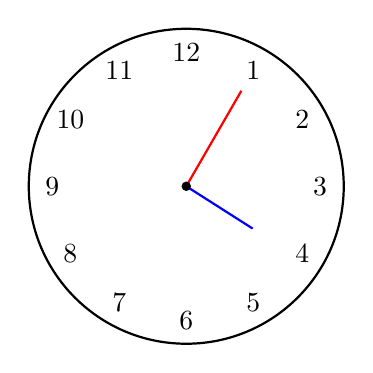
\begin{tikzpicture}[scale=2]
  % Draw the clock circle
  \draw[thick] (0,0) circle(1);

  % Place hour numbers
  \foreach \num in {1,...,12} {
    \node at ({90-30*\num}:0.85) {\num};
  }

  % Minute hand (5 minutes -> at "1")
  \draw[thick, red] (0,0) -- ({90-30*1}:0.7);

  % Hour hand (4 hours + 5 minutes -> 4*30 + 2.5 = 122.5 degrees clockwise)
  \draw[thick, blue] (0,0) -- ({90-(4*30+2.5)}:0.5);

  % Center dot
  \fill (0,0) circle(0.03);
\end{tikzpicture}
\end{center}
\end{enumerate}
\end{example}

\begin{exercise}
Which of the following relations are not equivalent relations and why?
\begin{enumerate}
\item $a\;R\;b$ if $a = b$.
\item $a\;R\;b$ if $a \leq b$.
\item $a\;R\;b$ if $gcd(a,b) = 1$.
\end{enumerate}
\end{exercise}

\subsection{Equivalence classes and partitions}
\label{sec:eq-classes}

\begin{theorem}
An equivalence relation defined on  set $A$  {\emph partitions} $A$ into disjoint equivalence classes: every element of $A$ belongs 
to exactly one equivalence class, and the classes together cover all of $A$.
\end{theorem}

\begin{proof}
We have to argue for two things -- first, no element belongs to two or more equivalent classes; and second, the union of all the equivalence classes covers the whole set.

Suppose $x$ belongs to two distinct equivalence classes. Then there exits $a,b \in A$ such that $x \sim a$ and $x \sim b$ but $a \not \sim b$. But this is not possible because $\sim$ is symmetric and transitive.

And, by reflexivity, each $x$ is at least equivalent to itself. So, no element is left out.
\end{proof}

\begin{example}
The relation Congruence of integers (mod $3$)  split $\Z$  into three classes:
\[
[0] = \{\dots,-6,-3,0,3,6,\dots\}, \quad
[1] = \{\dots,-5,-2,1,4,7,\dots\}, \quad
[2] = \{\dots,-4,-1,2,5,8,\dots\}.
\]
These three classes form a partition of $\Z$.
\end{example}

\section{Modular Arithmetic, Magic Squares, and One-Time Pads}
\label{sec:modular}

\subsection{Modular arithmetic}
Consider, for example, the set $\mathbb{Z}_7 = \{0,1,2,3,4,5,6\}$ consists of all integers modulo $7$. 
This means that we can perform addition and multiplication, and then reduce the result 
to its remainder upon division by $7$.

\paragraph{Addition.}
Examples:
\[
3 + 5 \equiv 1 \pmod{7}, \quad 6 + 4 \equiv 3 \pmod{7}.
\]

Every element has an \emph{additive inverse}, i.e.\ a number $x$ such that 
$a + x \equiv 0 \pmod{7}$. We denote this as $x \equiv a^{-1} \pmod{7}$
\[
0^{-1} \equiv 0 \pmod{7},\quad 1^{-1} \equiv 6 \pmod{7}, \quad 2^{-1} \equiv 5, \pmod{7},\quad 3^{-1} \equiv 4 \pmod{7},.
\]

\paragraph{Multiplication.}
Examples:
\[
3 \times 5 \equiv 1 \pmod{7}, \quad 4 \times 6 \equiv 3 \pmod{7}.
\]
For multiplication, every nonzero element has a \emph{multiplicative inverse}, 
i.e.\ $a \cdot x \equiv 1 \pmod{7}$.
\[
1^{-1} \equiv 1 \pmod{7},\quad 2^{-1} \equiv 4 \pmod{7},\quad 3^{-1} \equiv 5 \pmod{7},,\quad 6^{-1} \equiv 6 \pmod{7},.
\]
Notice that $0$ has no multiplicative inverse.

Thus $(\mathbb{Z}_7, +)$ is a finite arithmetic structure under addition, 
and $(\mathbb{Z}_7^\times,\cdot)$ with $\{1,2,3,4,5,6\}$ is a finite arithmetic structure under multiplication. This has many interesting applications.

\subsection{Magic Squares}
A \emph{magic square} is an arrangement of numbers in a square grid such that the sums of each row, column, 
and both diagonals are the same. Modular arithmetic allows us to construct magic squares 
in structures like $\mathbb{Z}_n$, where the “magic sum” is computed modulo $n$.  
This is a playful illustration of modular addition applied to combinatorial design. 

A simple way to build a magic square \emph{modulo $n$} is to take any ordinary magic square
and reduce each entry modulo $n$. The \href{https://en.wikipedia.org/wiki/Luoshu\_Square}{LuoShu $3\times 3$ square}, which has a rich history in occult and numerology is given as
\[
\begin{array}{|c|c|c|}
\hline
4 & 9 & 2 \\
\hline
3 & 5 & 7 \\
\hline
8 & 1 & 6 \\
\hline
\end{array}
\qquad\text{(each line sums to $15$)}
\]
It reduces modulo $7$ to
\[
\begin{array}{|c|c|c|}
\hline
4 & 2 & 2 \\
\hline
3 & 5 & 0 \\
\hline
1 & 1 & 6 \\
\hline
\end{array}
\quad\in\; \mathbb{Z}_7^{\,3\times 3}.
\]
Since $15\equiv 1\pmod{7}$, every row, column, and diagonal now sums to $\overline{1}\in\mathbb{Z}_7$.
For instance,
\[
4+2+2 \equiv 8 \equiv 1 \pmod{7},\qquad
3+5+0 \equiv 8 \equiv 1 \pmod{7},\qquad
1+5+2 \equiv 8 \equiv 1 \pmod{7}.
\]
The diagonals also satisfy $4+5+6\equiv 15\equiv 1\pmod{7}$ and $2+5+1\equiv 8\equiv 1\pmod{7}$.

\paragraph{General recipe (odd moduli).}
Let $S$ be any $3\times 3$ magic square over the integers with magic sum $M$.
For any modulus $n\ge 2$, the entry-wise reduction $\overline{S}\in(\mathbb{Z}_n)^{3\times 3}$ is a
magic square in $\mathbb{Z}_n$ with magic sum $\overline{M}\in\mathbb{Z}_n$,
because modular addition preserves equality of sums. More generally, for any $\alpha,\beta\in\mathbb{Z}_n$,
the entry-wise  transform $\alpha S+\beta$ is again a magic square modulo $n$ with magic sum
$\alpha M+3\beta \pmod{n}$.

\subsection{Perfect Secrecy and One-Time Pads}
The idea of modular arithmetic is also central in cryptography.  
In the \emph{one-time pad}, a message (plaintext) is converted into numbers 
(say letters $A=0,\dots,Z=25$). A random secret key of the same length is chosen, 
and encryption is done by addition modulo $26$:
\[
\text{ciphertext}_i \equiv \text{plaintext}_i + \text{key}_i \pmod{26}.
\]
Decryption uses subtraction modulo $26$.  

Claude Shannon showed that if the key is truly random, used only once, and kept secret, 
then the ciphertext reveals no information about the plaintext: this is called 
\emph{perfect secrecy}. Thus, a simple application of modular addition gives us 
a theoretically unbreakable cryptosystem.

\subsection*{Summary}
Modular arithmetic provides the framework to work with remainders in a structured way. 
It underlies recreational mathematics like magic squares, as well as fundamental 
cryptographic protocols such as the one-time pad.


\section*{Problems}

\begin{enumerate}

  \item Let $A = \{1,2,3\}$ and $B = \{a,b,c\}$.  
  (a) List all elements of the Cartesian product $A \times B$.  
  (b) Define two different binary relations $R_1, R_2 \subseteq A \times B$.  
  (c) Which of them, if any, are functions?

  \item Show that the relation $\leq$ on $\mathbb{N}$ is a subset of $\mathbb{N} \times \mathbb{N}$.  
  Explicitly write out the first ten elements of this relation.

  \item Give an example of a relation from $\{1,2,3\}$ to $\{a,b\}$ that is not a function.  
  Explain why it fails to satisfy the definition of a function.

  \item Consider the function $f : \mathbb{N} \to \mathbb{N}$ defined by $f(n) = 2n$.  
  Argue that $f$ is injective but not surjective.  

  \item Consider the function $g : \mathbb{N} \to \mathbb{N}$ defined by  
  \[
    g(0) = 0, \qquad g(n) = n-1 \ \text{for } n > 0.
  \]
  Show that $g$ is surjective but not injective.  

  \item Let $h : \mathbb{Z} \to \mathbb{Z}$ be defined by $h(x) = x+5$.  
  Prove that $h$ is bijective and describe its inverse function.

  \item Define the function $p : \mathbb{N} \times \mathbb{N} \to \mathbb{N}$ by $p(a,b) = a \times b$.  
  Argue formally that $p$ is a well-defined function.

  \item Construct an example of a function $f : A \to B$ where $A = \{1,2,3,4\}$, $B = \{a,b\}$ 
  that is neither injective nor surjective. Explain why.

  \item Prove that if a function $f : A \to B$ is bijective, then there exists a unique inverse 
  function $f^{-1} : B \to A$ such that $f^{-1}(f(a)) = a$ for all $a \in A$.  

  \item Consider the function $f : \mathbb{N} \to \mathbb{N}$ defined recursively as  
  \[
    f(0) = 0, \quad f(n+1) = f(n) + (2n+1).
  \]
  Show that $f(n) = n^2$. What kind of function is this (injective, surjective, bijective)?  

  \item Give an everyday example (outside mathematics) of:  
  (a) an injective mapping,  
  (b) a surjective mapping, and  
  (c) a bijective mapping.  

  \item Challenge: Prove or disprove — the composition of two injective functions is injective, 
  and the composition of two surjective functions is surjective. What about bijective functions?  
  
  % Equivalence relations
  \item On the set $\{1,2,3,4,5,6\}$, define a relation $R$ by $a \sim b$ if $a-b$ is divisible by $2$. 
        \begin{enumerate}
            \item Show that $R$ is an equivalence relation.
            \item List the equivalence classes.
        \end{enumerate}

  \item Consider the relation ``$x$ has the same number of letters as $y$'' on the set of English words.
        Prove or disprove that it is an equivalence relation. What do the equivalence classes look like?

  % Modular arithmetic
  \item Work out the addition and multiplication tables of $\mathbb{Z}_5$. Identify all additive and multiplicative inverses.

  \item In $\mathbb{Z}_7$, solve the linear congruence $3x \equiv 2 \pmod{7}$.

  \item Find all solutions to $x^2 \equiv 1 \pmod{15}$. 

  % Bijections and countability
  \item Construct a bijection between the set of even numbers and $\mathbb{N}$. 
        Then, using a diagram, show how integers $\mathbb{Z}$ can be listed in sequence, proving that they are countable.

%  \item Use Cantor’s diagonal method to prove that the real numbers in $[0,1]$ are uncountable. Illustrate with a decimal expansion example.

  \item Show that the set of rational numbers $\mathbb{Q}$ is countable by describing an explicit enumeration strategy.

  % Magic squares and applications
  \item Verify that the LuoShu square
        \[
        \begin{array}{|c|c|c|}
        \hline
        4 & 9 & 2 \\
        \hline
        3 & 5 & 7 \\
        \hline
        8 & 1 & 6 \\
        \hline
        \end{array}
        \]
        is a magic square. What is its magic sum?

  \item Construct a $3\times 3$ magic square modulo $7$ using the method of reducing an ordinary magic square.
        What is the magic sum in $\mathbb{Z}_7$?

  % Cryptography
  \item In a one-time pad over the alphabet $\{A=0,B=1,\dots,Z=25\}$, encrypt the message 
        \texttt{MATH} with the key \texttt{CODE}. 
        Show the numerical steps modulo $26$ and give the ciphertext.

  \item Explain why re-using the same key in a one-time pad scheme can destroy perfect secrecy. 
        Give a simple example with short  strings.


\end{enumerate}
